\chapter{Darwin Library}
\label{sec:darwin_lib}

Darwin is a simple library written in Python for BN modeling and inference.
The main purpose of the library is teaching BNs and quick prototyping or testing small networks.
In order to achieve these goals, the library has a simplistic approach of implementation, using native Python data structure and light usage of object oriented programming.
The structure of Darwin is basically divided into two categories: potentials and graph manipulations.
The features are also split into two main categories: inference and modeling tools.
Later, in this section, we also present a guide for getting started using Darwin.

\section{Structure}
\label{sec:system:sec1}

In order to work with BNs, Darwin has two main set of implementations: potential and graph manipulations.
These two categories form individually or together the tree structure of the library as presented in Figure \ref{fig:tree_darwin}.

\begin{figure}[hbt]
    \begin{center}
        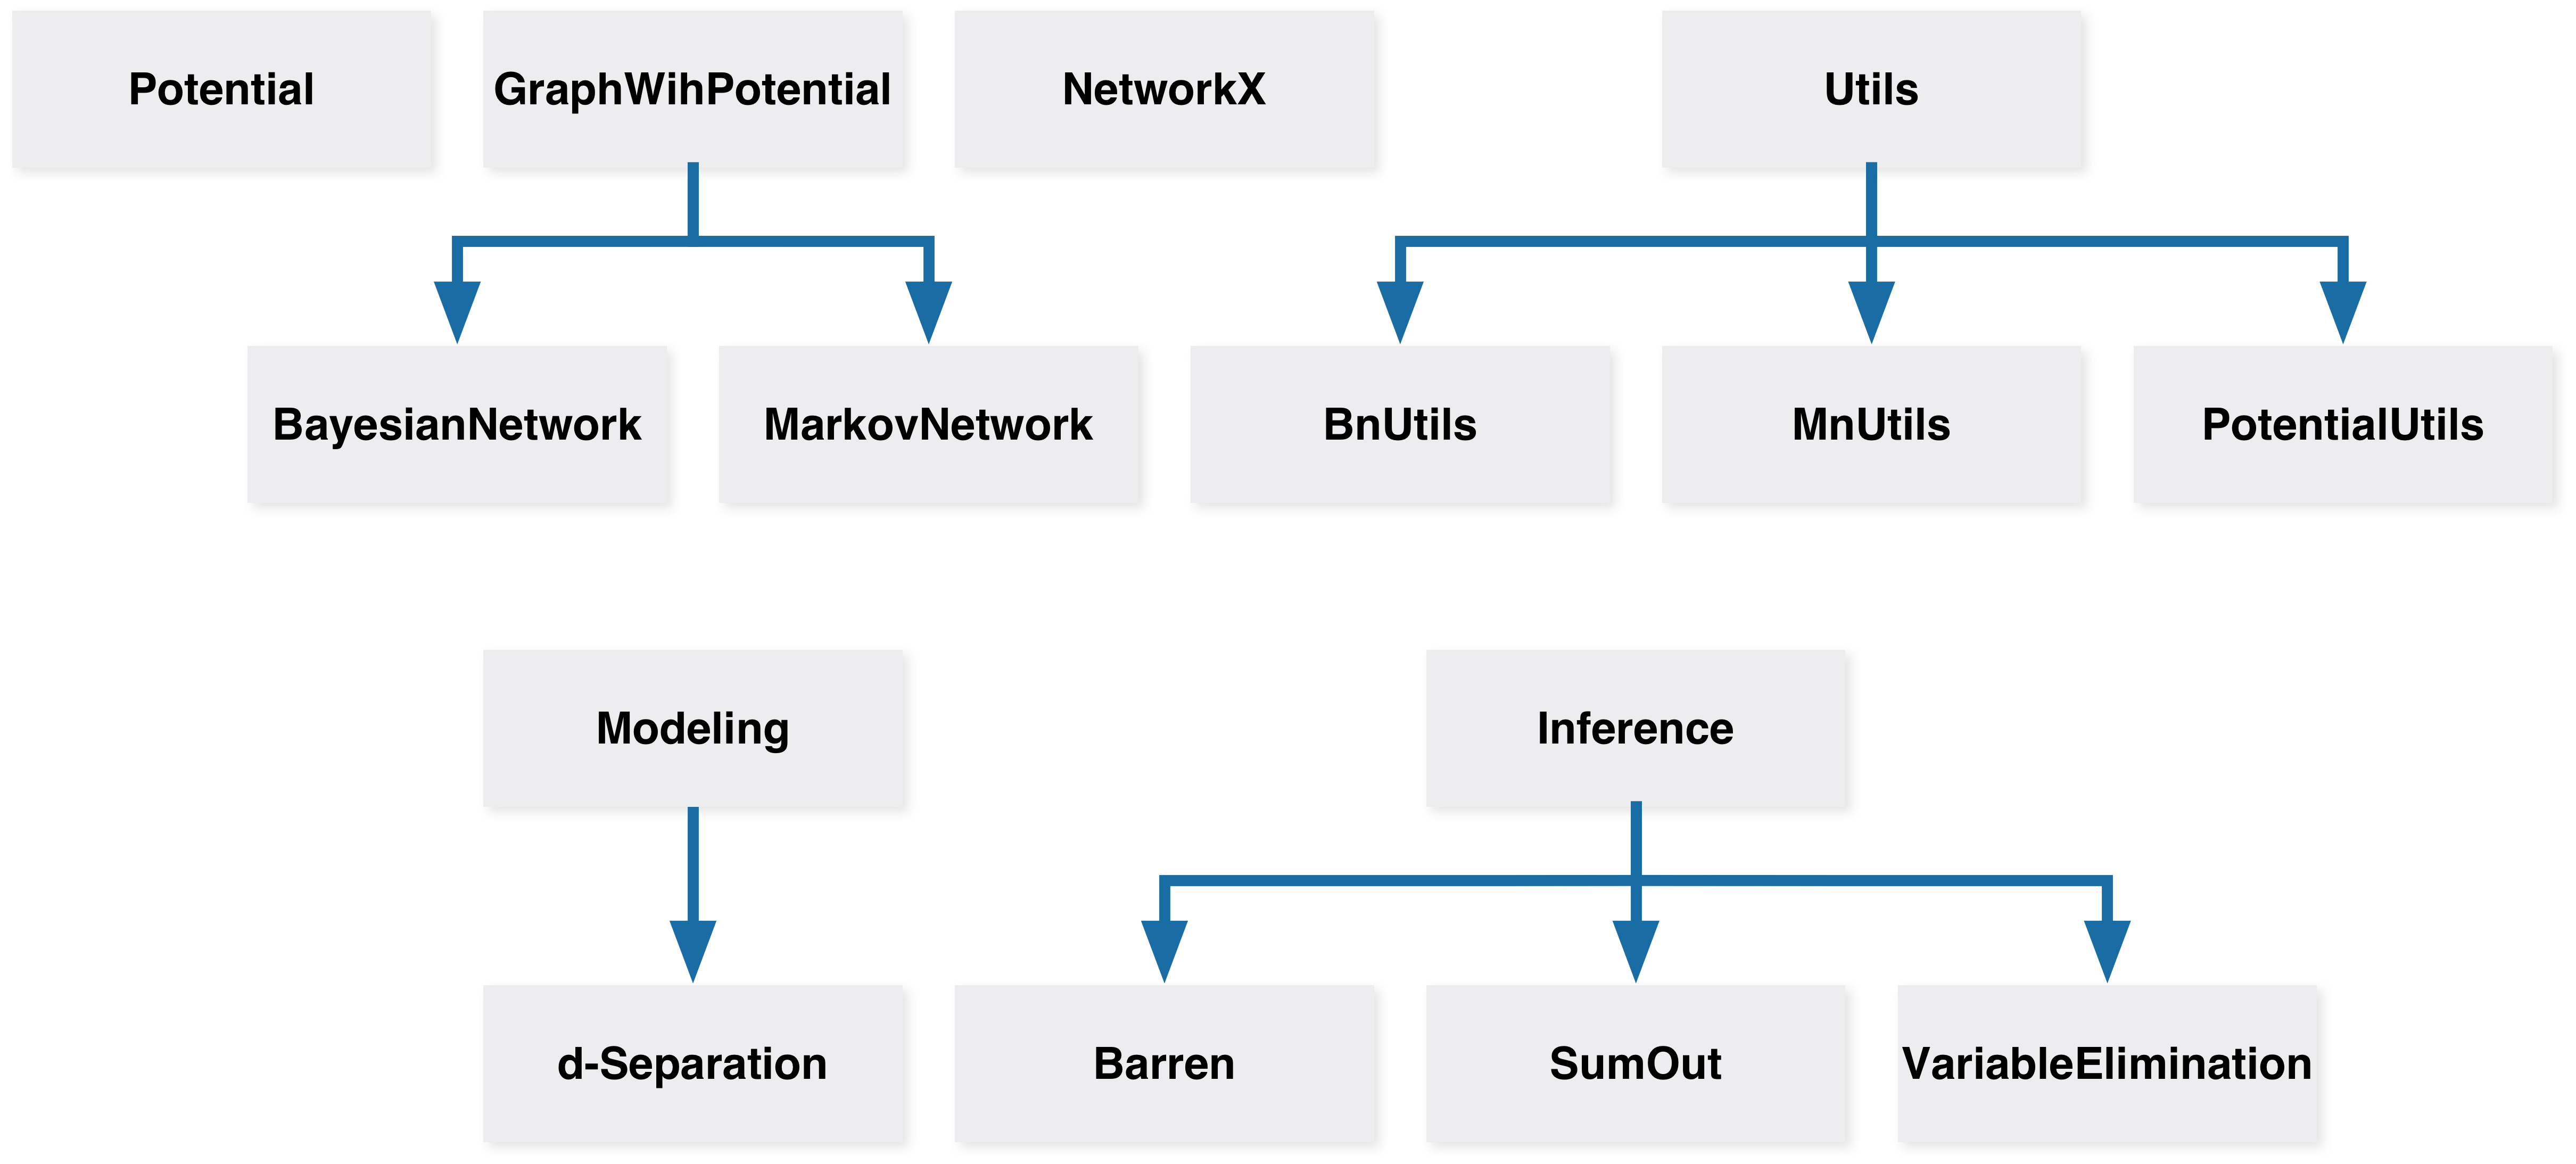
\includegraphics[width=\textwidth]{img/structure_darwin}
    \end{center}
    \caption{Three structure of Darwin.}
    \label{fig:tree_darwin}
\end{figure}

At the root, the class \emph{Potential} is a data structure for modeling a probability table.
The \emph{NetworkX} \cite{hagberg-2008-exploring} is set of data structures for graph manipulation and is also included at the root of the library.
Similarly, \emph{GraphWithPotential} is a class which basically maps nodes in a graph with a set of potentials, besides providing manipulations on the graph and the potentials on it.
\emph{BayesianNetwork} is a class that inherits from \emph{GraphWithPotential} but maps only one potential per node.
This data structure is used for modeling a BN.
In the same way, the class \emph{MarkovNetwork} entirely inherits the behaviour and properties of \emph{GraphWithPotential}, therefore it can be used for MN modeling.

The \emph{Utils} branch is formed by a set of standalone functions which implement core procedures for the other classes.
Mainly, these functions are defined by numerical operations on lists of probabilities.
One advantage of having those implementations as standalone functions is that future optimized code can be included or modified without disturbing the other classes, since the other classes only makes a function call to those utilities functions.
Basically, there are three main utilities: \emph{BnUtils}, \emph{MnUtils}, and \emph{PotentialUtils}.
The BnUtils has a set of functions for BN manipulations and operations, such as moralization, triangulization, join tree construction, among others.
In MnUtils, we have utilities for MN propagation such as finding an optimal path for propagating in a tree.
Lastly, PotentialUtils is formed by a set of procedures for numerical operations such as multiplication, division and marginalization of tables.
All potential manipulations in PotentialUtils is implemented according to the efficient implementation proposed in \cite{koll09}.

In the \emph{Modeling} brach, there is an implementation of d-Separation as proposed in Algorithm 3.1 of \cite{koll09}.
While in the branch \emph{Inference} there are few data structures useful for exact inference in BNs.
The \emph{Barren} function is used for identifying barren potentials in factorizations.
\emph{SumOut} is a function which systematically removes a set of variables from a factorization by multiplying potentials with the variables and them marginalizing the variables out.
The class \emph{VariableElimination} implements the exact inference algorithm VE as originally proposed by \cite{zhan94}.
Finally, the \emph{Test} branch has a set of unit tests which assure the correct functioning of core functions in the whole library.

\section{Features}
\label{sec:system:sec2}

Here, we highlight some feature of the library.
In general, the features are tools to facilitate the use of Darwin in teaching and prototyping of small system.
The library is not intended for fast inference, neither high accuracy.
Therefore, all numerical operations are implemented using native Python code, instead of high performance libraries such as \emph{numpy} \cite{van2011numpy}.
The graph manipulations are done by an external library called \emph{NetworkX}, a robust and well known library with high performance and large set of tools.

For modeling, Darwin has the testing of d-Separation implemented using a reachability algorithm.
Also, the library has built in tools for converting a BN into a MN, including the join tree construction by moralization, triangulization and the assignment of potentials.
The triangulization step, specifically, has implemented 4 different heuristics, the same as implemented in \emph{PgmPy} \footnote{http://pgmpy.org}.

For inference, the library provides a basic function for eliminating variables in a factorization, called \emph{SumOut}.
But for faster inference, it is recommended to use the VE implementation which absorb evidence, removes barren and independent by evidence potentials, perform inference by summing out non relevant variables and, finally, normalize the final result.

\section{Usage}
\label{sec:system:sec3}

In order to get started with Darwin, we now present a quick overview of the most common classes and functions.
The main classes are \emph{Potential}, \emph{GraphWithPotential}, \emph{BayesianNetwork}, and \emph{MarkovNetwork}.

The Potential class is defined by the given arguments: \emph{variables} which is a list with strings, \emph{cardinalities} corresponding to the variables which is a list with integers in the same order than the variables, probabilities \emph{values} in a list with floating numbers, \emph{left hand side} which is a list with the variables in the LHS of the potential, and similarly the \emph{right hand side} is defined.
For example, considering a CPT $P(a|b)$ with binary variables and probability values 0.4, 0.5, 0.6, 0.5, we can use Darwin to represent this potential as:
\begin{verbatim}
    Potential(["a", "b"], [2, 2], [0.4, 0.5, 0.6, 0.5], ["b"], ["a"])
\end{verbatim}

The GraphWithPotential class contains basically a list with potentials, a graph defined using NetworkX, and a dictionary mapping nodes in the graph to a list of potentials.
After declaring a GraphWithPotential, the user can add potentials to a node using the \emph{add\_potential} method.
For example, the following code creates a graph with two nodes $\{a\}$ and $\{a,b\}$ and assign $P(a)$ to $\{a\}$ and $P(b|a)$ to $\{a,b\}$ in a GraphWithPotential.
\begin{verbatim}
    p1 = Potential(["a"], [2], [0.2, 0.8], ["a"], [])
    p2 = Potential(["a", "b"], [2, 2], [0.4, 0.5, 0.6, 0.5], ["b"], ["a"])
    
    G = networkx.Graph()
    G.add_nodes(["a", "ab"])
    
    GwP = GraphWithPotential()
    GwP.add_potential("a", p1)
    GwP.add_potential("ab", p2)
\end{verbatim}

The MarkovNetwork inherits from GraphWithPotential, therefore modeling a MN is simply using the GraphWithPotential like in the code above.
In the same way, modeling a BN uses the BayesianNetwork class which also inherits from GraphWithPotential.
The difference for a BN is that only one potential is assigned at one node and the graph used is a DAG.
For instance, the code above can be used to declare a BN with two nodes $a \rightarrow ab$ just by changing the definition of $G$ to the below code, which is a directed graph.
\begin{verbatim}
    G = networkx.DiGraph()
    G.add_edge("a", "ab")
\end{verbatim}
